\documentclass{article}
%\usepackage[margin=1in]{geometry}
\usepackage{graphicx} % Required for inserting images
\usepackage{hyperref}
\usepackage{amsmath}
\usepackage{titling}
\usepackage{enumitem}
\usepackage{makecell}
\usepackage{minted}
\usepackage{url}
\usepackage{tabularx}
\usepackage{graphicx}
\renewcommand\maketitlehooka{\null\mbox{}\vfill}
\renewcommand\maketitlehookd{\vfill\null}

\begin{document}
\centering

\title{\Huge Intro Deep Learning Homework 1}

\author{ \huge
Jaskin Kabir \\
\Large Student Id: 801186717 \\
\Large \href{https://github.com/jaskinkabir/Intro_Deep_Learning/tree/master/HM1}{GitHub:}\\\url{https://github.com/jaskinkabir/Intro_Deep_Learning/tree/master/HM1}
}

\date{January 2025}

\begin{titlingpage}
\maketitle
\end{titlingpage}

\section{Problem 1: Character Prediction Small Dataset}

\begin{enumerate}[label=1\alph*. ]
    \item \textit{Training Curves}
    \begin{figure}[htb]
        \setkeys{Gin}{width=\linewidth}
        \setlength\tabcolsep{2pt}
        \begin{tabularx}{\textwidth}{XXX}
          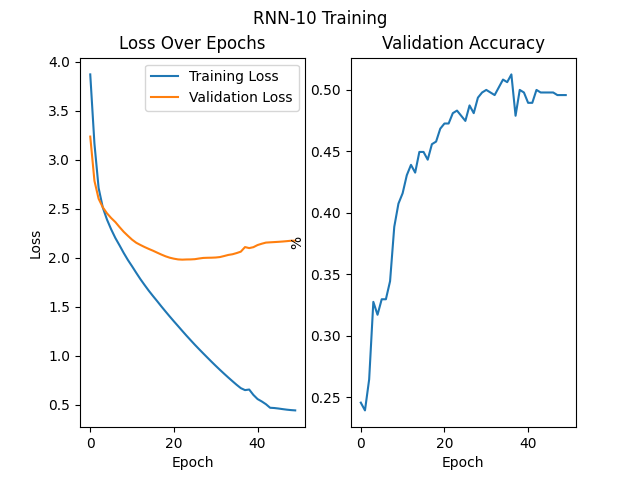
\includegraphics{images_p1/RNN_10_training_new.png} &
          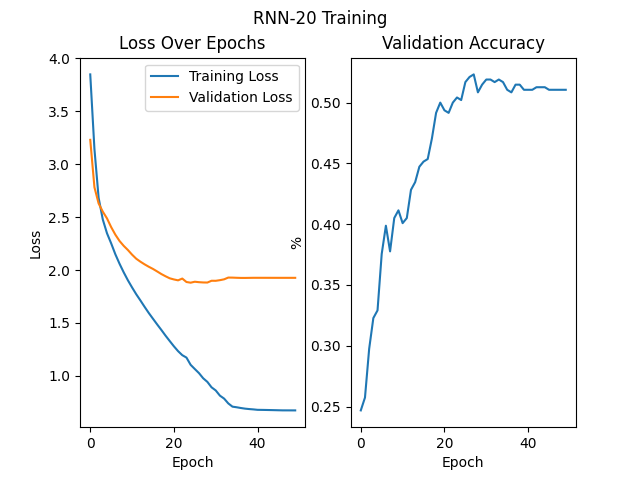
\includegraphics{images_p1/RNN_20_training_new.png} &
          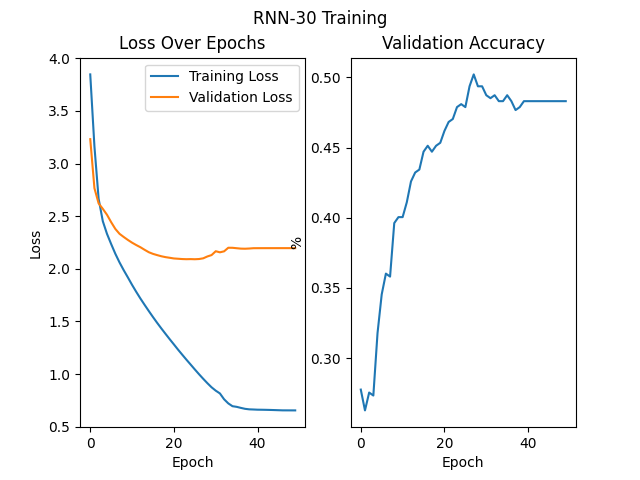
\includegraphics{images_p1/RNN_30_training_new.png}   \\
          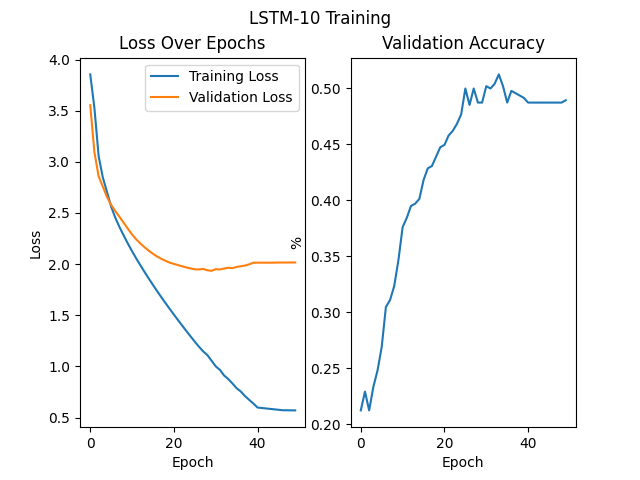
\includegraphics{images_p1/LSTM_10_training_new.png} &
          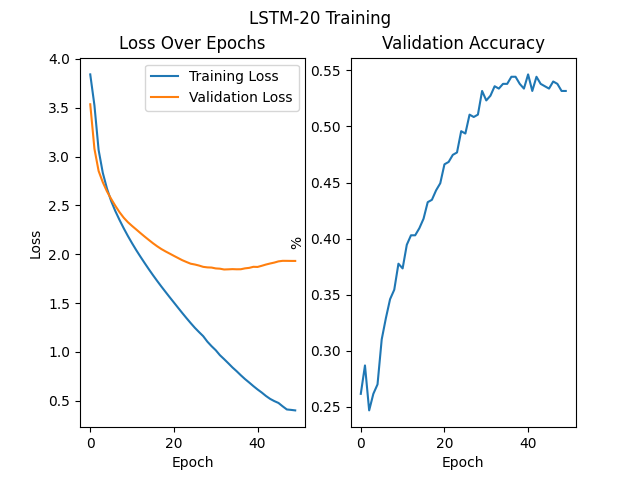
\includegraphics{images_p1/LSTM_20_training_new.png} &
          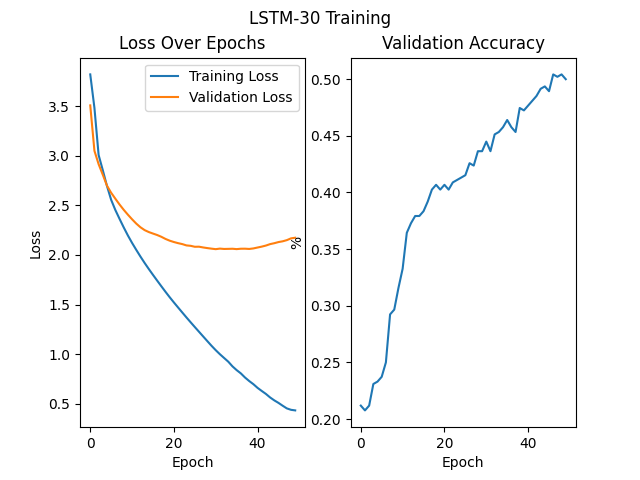
\includegraphics{images_p1/LSTM_30_training_new.png}   \\
          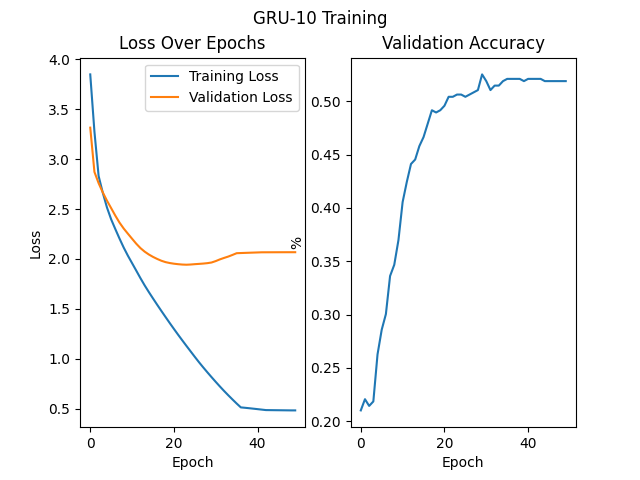
\includegraphics{images_p1/GRU_10_training_new.png} &
          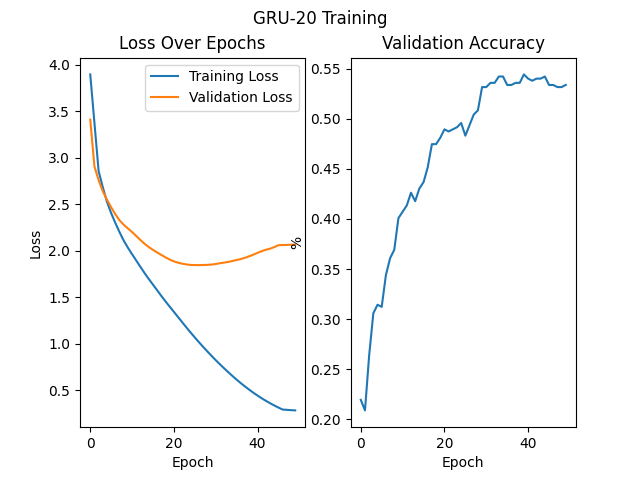
\includegraphics{images_p1/GRU_20_training_new.png} &
          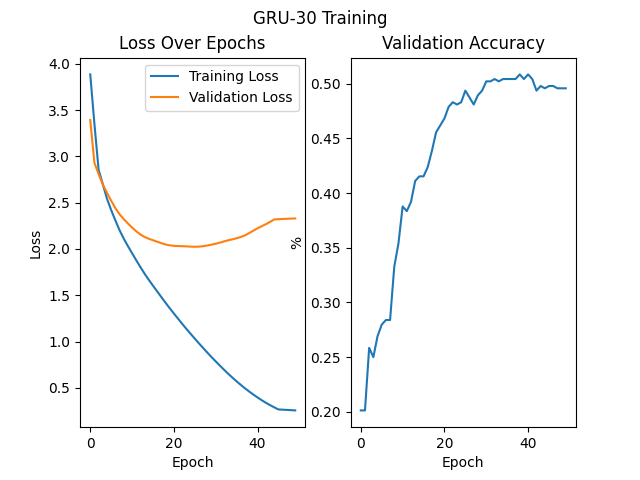
\includegraphics{images_p1/GRU_30_training_new.png}
        \end{tabularx}
        \caption{Problem 1 Training Curves}
        \label{fig:p1}
      \end{figure}
      \newpage
    \item \textit{Results Comparison}
    \begin{table}[h]
        \centering
        \renewcommand{\arraystretch}{1.5}
        \begin{tabular}{|>{\centering\arraybackslash}m{3cm}|>{\centering\arraybackslash}m{3cm}|>{\centering\arraybackslash}m{3cm}|>{\centering\arraybackslash}m{3cm}|>{\centering\arraybackslash}m{3cm}|}
        %\begin{tabular}{|l|r|r|r|r|}
            \hline
            \textbf{Model} & \textbf{Parameter Count} & \textbf{Training Time (s)} & \textbf{Overfit (\%)} & \textbf{Accuracy (\%)} \\
            \hline
            \textbf{RNN-10}  & 44846  & 1.93  & 389.68  & 49.58 \\
            \textbf{RNN-20}  & 44846  & 3.65  & 185.97  & 51.05 \\
            \textbf{RNN-30}  & 44846  & 5.24  & 235.41  & 48.31 \\
            \hline
            \textbf{LSTM-10} & 143918 & 5.79  & 253.80  & 48.95 \\
            \textbf{LSTM-20} & 143918 & 11.21 & 381.00  & 53.16 \\
            \textbf{LSTM-30} & 143918 & 18.23 & 399.18  & 50.00 \\
            \hline
            \textbf{GRU-10}  & 110894 & 5.30  & 329.01  & 51.89 \\
            \textbf{GRU-20}  & 110894 & 9.88  & 347.95  & 54.01 \\
            \textbf{GRU-30}  & 110894 & 15.41 & 460.00  & 50.85 \\
            \hline
        \end{tabular}
        \caption{Problem 1 Data Comparison}
        \label{tab:p1}
    \end{table}
    \item \textit{Discussion} 
    \begin{itemize}
        \item Parameter Count
            
            The parameter count of the LSTM network was more
            than triple that of the basic RNN network, and
            the GRU was almost halfway between the two. This
            is to be expected, as the LSTM adds significant
            complexity to the base RNN architecture, and the
            GRU reduces that complexity. This complexity
            comes from the number of gates in each
            architecture. 
        \item Training Time
        
            The RNN was the quickest to train, followed by
            the GRU and then the LSTM. Training time seemed
            to increase linearly with sequence length for
            all architectures.
        \item Effect of Sequence Length

            The sequence length of 10 was too short for the
            models to have enough relevant information,
            while the length of 30 was too difficult for the
            models to learn. The sequence length of 20 was
            the best compromise between the two. 

        \item Overfitting
        
            For the best sequence length of 20, the RNN had
            the lowest overfit and the LSTM the highest. This
            is likely a result of the difference in
            complexity between the architectures. The most
            complex model, the LSTM, had the highest
            overfit.

            Interestingly, for the sequence length of 10,
            the RNN the highest overfit while the LSTM had
            the lowest. This could be due to the RNN not
            having enough information to memorize the
            training data, while the LSTM was able to
            memorize more from the shorter sequences.

            For the sequence length of 30, the GRU had the
            highest overfit and the RNN the lowest. As the
            GRU was the most effective at generalizing from
            the training data, it makes sense that it would
            also overfit the most
        
        \item Accuracy
        
            Across all sequence lengths, the GRU was the
            most accurate and the RNN the least. The LSTM
            was in the middle. This is likely due to the
            complexity of the LSTM and the simplicity of the
            RNN. The GRU is a good compromise between the
            two, which is why it performed the best.

    
    \end{itemize}

\end{enumerate}
\newpage
\section{Problem 2: Shakespeare Character Prediction}
\begin{enumerate}[label=1\alph*. ]
    \item \textit{Training Curves}
    \begin{figure}[htb]
        \setkeys{Gin}{width=\linewidth}
        \setlength\tabcolsep{0.5pt}
        \renewcommand{\arraystretch}{0}
        \begin{tabularx}{\textwidth}{XXX}
          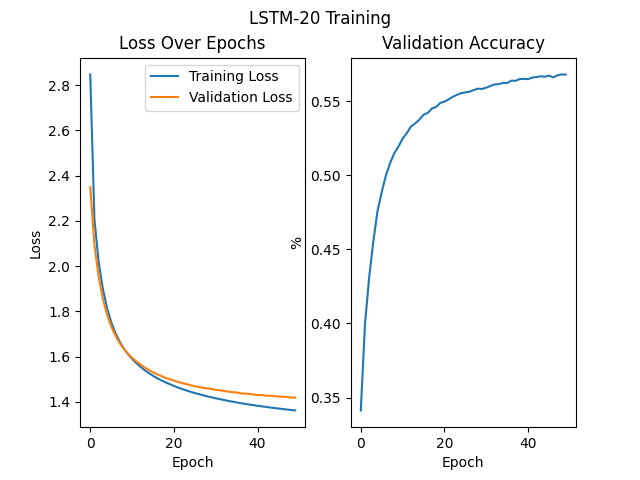
\includegraphics{images/LSTM-20_training_new.png} &
          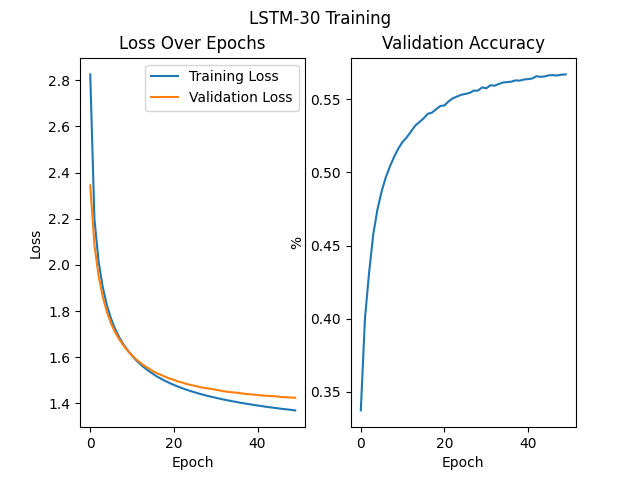
\includegraphics{images/LSTM-30_training_new.png} &
          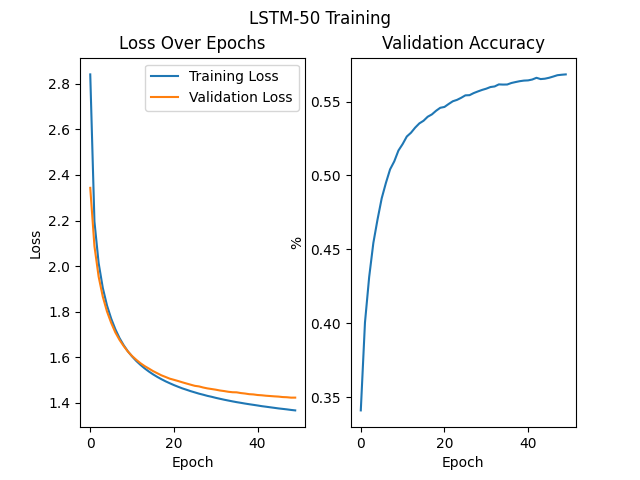
\includegraphics{images/LSTM-50_training_new.png} \\
          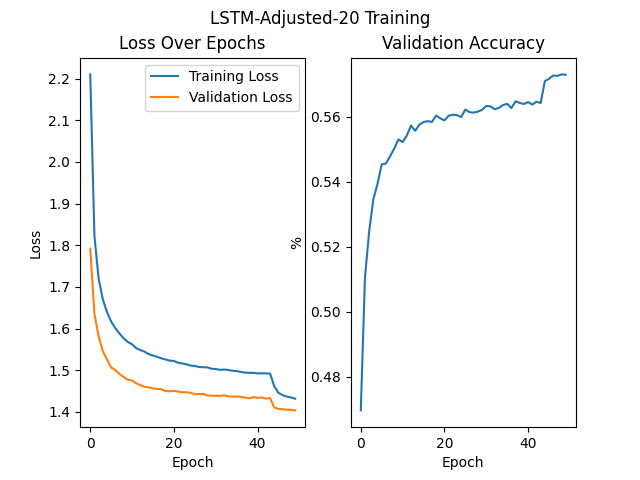
\includegraphics{images/LSTM-Adjusted-20_training_new.png} &
          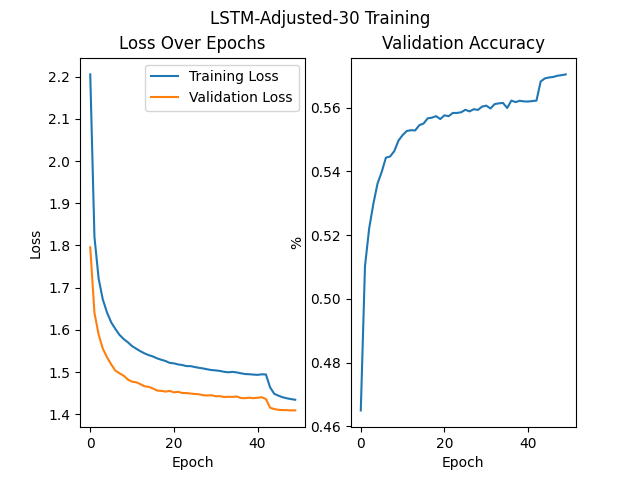
\includegraphics{images/LSTM-Adjusted-30_training_new.png} &
          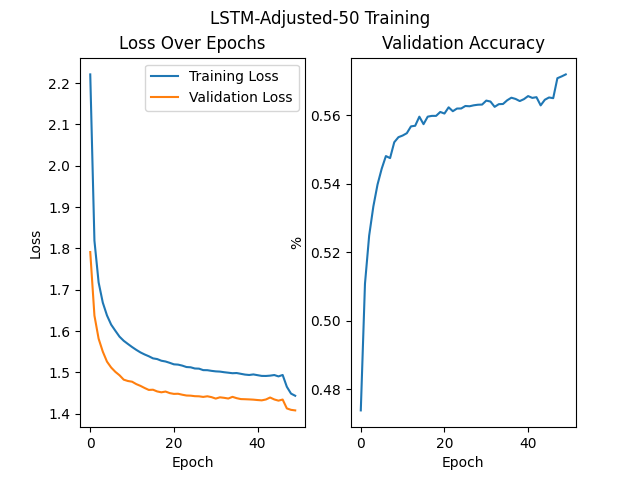
\includegraphics{images/LSTM-Adjusted-50_training_new.png} \\
          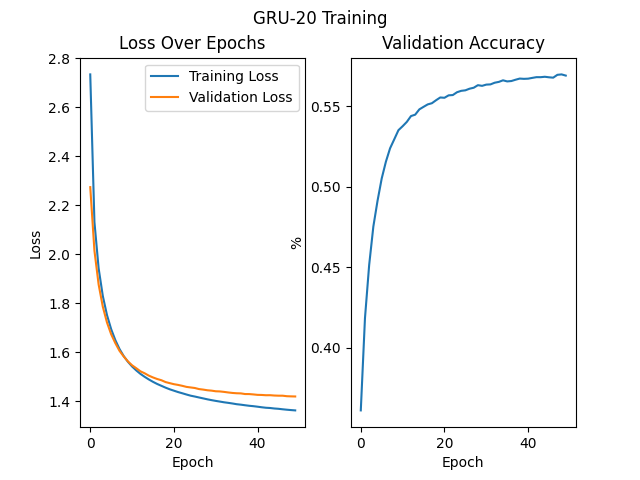
\includegraphics{images/GRU-20_training_new.png} &
          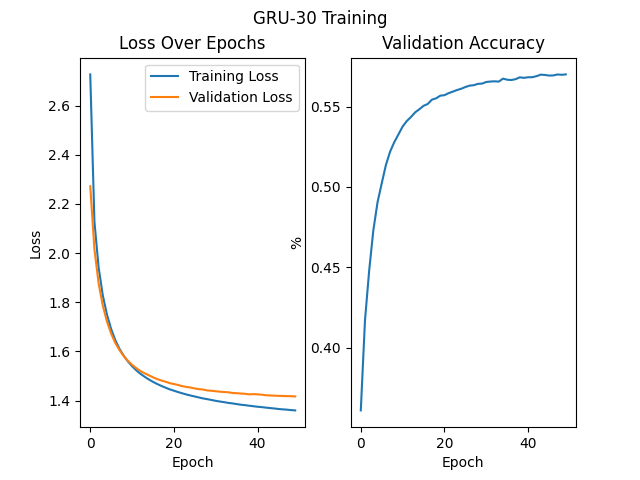
\includegraphics{images/GRU-30_training_new.png} &
          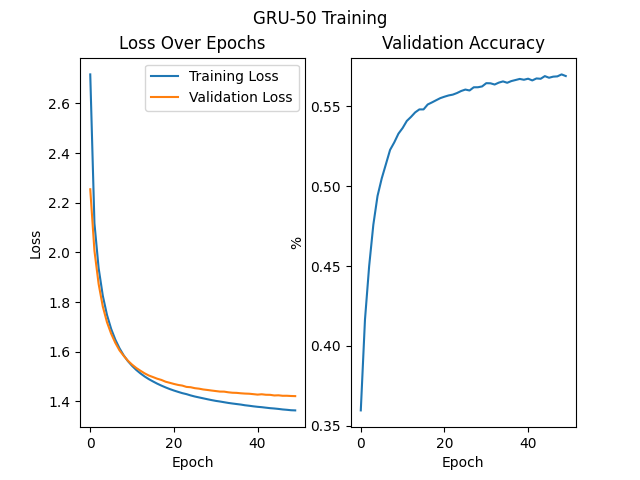
\includegraphics{images/GRU-50_training_new.png} \\
          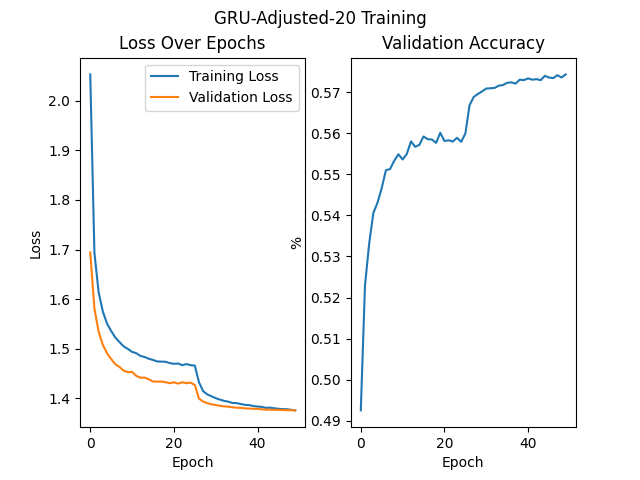
\includegraphics{images/GRU-Adjusted-20_training_new.png} &
          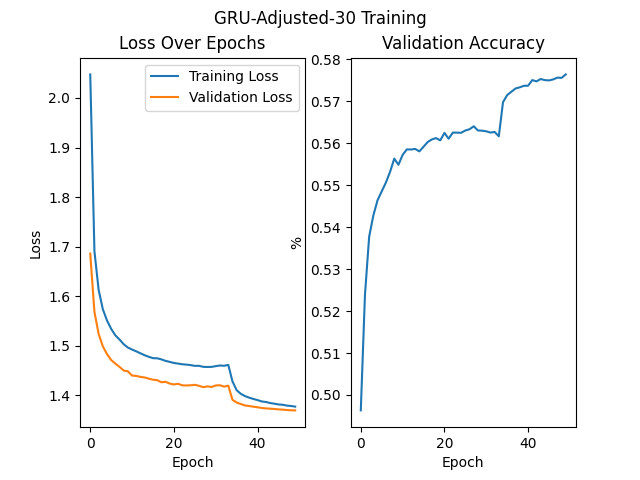
\includegraphics{images/GRU-Adjusted-30_training_new.png} &
          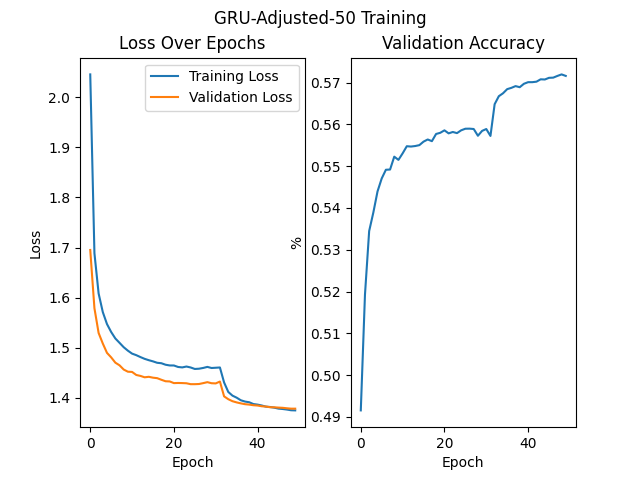
\includegraphics{images/GRU-Adjusted-50_training_new.png}
        \end{tabularx}
        \caption{Problem 2 Training Curves}
        \label{fig:p2}
      \end{figure}
      \newpage
    \item \textit{Results Comparison}
    \begin{table}[h]
        \centering
        \renewcommand{\arraystretch}{1.5}
        \begin{tabular}{|>{\centering\arraybackslash}m{3cm}|>{\centering\arraybackslash}m{3cm}|>{\centering\arraybackslash}m{3cm}|>{\centering\arraybackslash}m{3cm}|>{\centering\arraybackslash}m{3cm}|>{\centering\arraybackslash}m{3cm}|}
        %\begin{tabular}{|l|r|r|r|r|}
            \hline
            \textbf{Model} & \textbf{Parameter Count} & \textbf{Training Time (s)} & \textbf{Inference Time (s)} & \textbf{Overfit (\%)} & \textbf{Accuracy (\%)} \\
            \hline
            \textbf{LSTM-20}  & 148801   & 346.11  & 3.83  & 56.62 \\ %done
            \textbf{LSTM-30}  & 44846  & 3.65  & 185.97  & 51.05 \\
            \textbf{LSTM-50}  & 44846  & 5.24  & 235.41  & 48.31 \\
            \hline
            \textbf{LSTM-Adjusted-20} & 143918 & 5.79  & 253.80  & 48.95 \\
            \textbf{LSTM-Adjusted-30} & 143918 & 11.21 & 381.00  & 53.16 \\
            \textbf{LSTM-Adjusted-50} & 143918 & 18.23 & 399.18  & 50.00 \\
            \hline
            \textbf{GRU-20}  & 115777  & 5.30  & 329.01  & 51.89 \\
            \textbf{GRU-30}  & 110894 & 9.88  & 347.95  & 54.01 \\
            \textbf{GRU-50}  & 110894 & 15.41 & 460.00  & 50.85 \\
            \hline
            \textbf{GRU-Adjusted-20}  & 110894 & 5.30  & 329.01  & 51.89 \\
            \textbf{GRU-Adjusted-30}  & 110894 & 9.88  & 347.95  & 54.01 \\
            \textbf{GRU-Adjusted-50}  & 110894 & 15.41 & 460.00  & 50.85 \\
            \hline
        \end{tabular}
        \caption{Problem 2 Data Comparison}
        \label{tab:p2}
    \end{table}
    \item \textit{Discussion} 
    \begin{itemize}
        \item Parameter Count
            
            The parameter count of the LSTM network was more
            than triple that of the basic RNN network, and
            the GRU was almost halfway between the two. This
            is to be expected, as the LSTM adds significant
            complexity to the base RNN architecture, and the
            GRU reduces that complexity. This complexity
            comes from the number of gates in each
            architecture. 
        \item Training Time
        
            The RNN was the quickest to train, followed by
            the GRU and then the LSTM. Training time seemed
            to increase linearly with sequence length for
            all architectures.
        \item Effect of Sequence Length

            The sequence length of 10 was too short for the
            models to have enough relevant information,
            while the length of 30 was too difficult for the
            models to learn. The sequence length of 20 was
            the best compromise between the two. 

        \item Overfitting
        
            For the best sequence length of 20, the RNN had
            the lowest overfit and the LSTM the highest. This
            is likely a result of the difference in
            complexity between the architectures. The most
            complex model, the LSTM, had the highest
            overfit.

            Interestingly, for the sequence length of 10,
            the RNN the highest overfit while the LSTM had
            the lowest. This could be due to the RNN not
            having enough information to memorize the
            training data, while the LSTM was able to
            memorize more from the shorter sequences.

            For the sequence length of 30, the GRU had the
            highest overfit and the RNN the lowest. As the
            GRU was the most effective at generalizing from
            the training data, it makes sense that it would
            also overfit the most
        
        \item Accuracy
        
            Across all sequence lengths, the GRU was the
            most accurate and the RNN the least. The LSTM
            was in the middle. This is likely due to the
            complexity of the LSTM and the simplicity of the
            RNN. The GRU is a good compromise between the
            two, which is why it performed the best.

    
    \end{itemize}

\end{enumerate}


\end{document}